\documentclass[parskip=full]{scrreprt}
% Paket um vordefinierte Texte (z.B. "Inhaltsverzeichnis") auf Deutsch zu übersetzen
\usepackage[english]{babel}

% Paket um Schriftarten festzulegen (für XeLaTeX)
\usepackage{fontspec}

% serifenfreie Schriftart Arial festlegen
% \setsansfont{}ð

% serifenfreie Schriftvariante verwenden
\renewcommand{\familydefault}{\sfdefault}

% Paket um Grafiken (JPG, PNG, PDF) einzubinden
\usepackage{graphicx}

% Paket für Zeilenabstand
\usepackage{setspace}

% Paket für korrekte Anführungszeichen
\usepackage{csquotes}

% Paket für selbst definierte Kopf- und Fusszeilen
\usepackage{scrlayer-scrpage}

% Pakte für Zitate und Bibliografie
\usepackage{biblatex}

\addbibresource{literature.bib}

% Paket zum Erzeugen von Platzhaltertext
\usepackage{lipsum}

% Code below courtesy of chatgpt-4o on 2024-06-25

% Package for changing theorem style
\usepackage{amsthm}

% Code to change theorem styling
\setlength{\topsep}{0.1em}
\setlength{\partopsep}{0.1em} % Extra space above theorem if at the beginning of a list
\setlength{\parsep}{0.1em} % Space between paragraphs within the theorem

% End of code courtesy of chatgpt-4o

% Packge for code highlighting
\usepackage{listings}


\usepackage{courier}        % For monospace font
\usepackage{xcolor}         % For background color

\lstdefinestyle{customverilog}{
    language=verilog,                    % Set language to Verilog/SystemVerilog
    basicstyle=\ttfamily\scriptsize,                % Monospace font
    breaklines=true,                     % Break long lines if necessary
    numbers=left,                        % Line numbers on the left
    numberstyle=\tiny,                   % Line numbers in tiny font
    backgroundcolor=\color{gray!10},     % Light gray background
}


\lstset{style=customverilog}


% Package for hyperlinks
\usepackage[hidelinks]{hyperref}

% Package for float placement
\usepackage{float}

% noitemsep
\usepackage{enumitem}
\setlist{nolistsep}
\setlist{noitemsep}

% tikz
\usepackage{tikz}
\usepackage{tikz-timing}
\usetikzlibrary{shapes.geometric, arrows.meta}
\usepackage{caption}
\DeclareCaptionType {timingdiag}[Timing diagram][List of Timing Diagrams]

\renewcommand*{\ttdefault}{cmtt}

% listings

% Schmale Seitenränder festlegen
\KOMAoption{DIV}{15}

% Text auf Titelseite festlegen
\subject{Maturapaper}
\title{Designing and Implementing an 8-bit Computer Architecture in SystemVerilog}
\author{Author Author}

\date{}

\publishers{Publisher Publisher}

% selbst definierte Kopf- und Fusszeile
\lohead{Matura paper}
%\rohead{\input{jobid}, \input{gitbranch.tex}@\input{githash}}
\rohead{Author Author}
\cofoot{\thepage}

% Zeilenabstand festlegen
\singlespacing
%\onehalfspacing
%\doublespacing

% Trennlinie für Kopfzeile
\KOMAoption{headsepline}{off} % oder on

% Trennlinie für Fusszeile
\KOMAoption{footsepline}{on} % oder on

\usepackage{comment}
\excludecomment{figure}
\let\endfigure\relax

\begin{document}


\maketitle
\textcopyright Rufus Spyra. 2024.

PERMISSION IS HEREBY GRANTED SOLELY FOR THE PURPOSE OF PLAGIARISM CHECKS ON IT. I DO NOT CONSENT TO ANY FURTHER STORAGE OR USAGE OF THIS DOCUMENT AFTER THE CHECK HAS BEEN COMPLETED. I DO NOT CONSENT TO ANY ANONYMIZATION.
\tableofcontents

\chapter{Introduction}
My fascination of retro computers sparked when I watched an online show about building an 8-bit computer on a breadboard. After countless hours of explanations, the viewer was rewarded with a blinking monster of wires and chips, functioning together to reach a goal. Ever since I watched this show \cite{beneater}, I wanted to design and build a computer like this. Over a couple of years I got further invested in the topic, fascinated by the initial impact of the first introduction of 8-bit computers in the 1970s and the sheer complexity of computer chips, I wanted to design my own computer architecture and simulation - just like if it was a real chip design, that is supposed to be physically manufactured on silicon. Unfortunately, physical construction, be it in silicon, or any other medium, was quickly ruled out due to overwhelming time efforts and costs. Manufacturing a chip in silicon not only requires physical manufacturing capabilities but also highly specialized software, that is proprietary and not intended for amateur usage. 

The goal of this project is to design a computer architecture following the process and constraints of a chip design up until silicon or hardware design and manufacturing.

Following my inspiration, the architecture that is to be designed shall be kept very simple. This is achieved by limiting the bus width to 8-bits. Furthermore, the architecture shall follow the classic von Neumann Architecture and be Turing equivalent.  


\section{Chip Design} \label{sec:chip-design}
To move from idea to a finished product, chip designs follow a specific flow. Although different sources may describe this process differently. It is clear however, that this process is intended to be highly sequential and linearized.

At first, all top level requirements must be clearly established, which are then further broken down in smaller and smaller requirements. This step is referred to as "System specification and architectural design".

At some point these requirements then reach the point where, they specify functional details of the chip/architecture, such as compartmentalization and signalling. This is then referred to as "Functional design." With enough specificity these requirements can then be transferred into computer aided designs utilizing hardware description computer languages, a process called "Logic design". This logic design can then be transferred, either manually or by sophisticated computer programs, into logic gates and a silicon layout, during the "physical design"  process. Before this is step is started, the logic design is tested against the defined requirements to ensure that it implements them correctly, which is called "Verification and Validation". Any mistakes in the logic design would translate into faulty silicon, making these mistakes extremely costly \cite{chipdesignflow1} \cite{chipdesignflow2}. The generated design would then be handed off to production.

As previously stated, this project shall treat all steps up until and with "Verification and Validation". The collection of this process is sometimes also referred to \textit{front end design}.

\subsection{Requirements}
\textit{Requirements engineering} describes the process of not only establishing high level requirements, e.g. the project goals, but also the translation into more specific and precise low level requirements. The formulation of useful requirements is essential to the success of a project. The value of a requirement lies in its ability to translate what the author wanted into what an engineer made of it. This means requirements must be unambiguous, correct and ideally precise and concise \cite{requirementsengineering}.

\subsection{Hardware Description Languages}
With the development of highly complex chip designs in the late 20th century, further and further abstraction of the logic design process was required, ensuring that all stakeholders knew the exact specifications of the design at any point. Whilst the earliest chip designs were drawn by hand and later transferred onto silicon by photolithography, chip designs nowadays are first written in an abstract computer language; a Hardware Description Language. This hardware description can then be transferred into silicon either manually or automatically.  Apart from also allowing separation, modularity and reusability of components, this description later also allowed for simulation of the design. This simulation brought the key advantage of being able to be tested against requirements to check for errors \cite{histverilog} \cite{1214355}.

\subsection{Automated Testing}
Nowadays, this automated testing process is handled by software frameworks designed for this purpose. These software frameworks instantiate and execute the simulation of the \textit{design under test} on top of \textit{testbench} code. The testbench models behaviour of external components which is applied onto the design under test. The response of it is then compared to expected results and validated to ensure the design meets all requirements.

While requirements should cover all of an architectures' logic design implementation, some pieces of code could be not covered by tests. To ensure that all code is tested, testing frameworks provide \textit{code coverage analysis tools}. The tools count activations of specific lines of code. This activation count can then be used to produce a visual report that shows all used lines of code, highlighting areas that aren't covered by test.

Automated testbenches can be generally be split into two categories: exhaustive testing and directed testing. Exhaustive testbenches test by supplying every possible test input to the design under test. Most of the time this is not required, as if it works for one input it should work for any other input. Exhaustive testing does also require significantly more time. Consequently, testbenches shall be written in a directed fashion. 

\cite{verilogtestbench} \cite{exhaustivetesting} \cite{directedtesting}


\subsection{Development Operations and Version Control Systems}
To track development over time \textit{version control systems} are used in basically every software project. Closely tied to most version control systems are \textit{development operations}. The goal of development operations is to connect the software development closer to its operations. In many projects these operations are e.g. the continuous deployment of code changes and the execution of automated tests. Applied to this project, the development operations signify the execution of automatic testing of code changes as soon as changes are registered with the version control system. 

This combination allows for tracking and tracing the development process over time and provides quick feedback to engineers on problems arising in the code.

\section{Computer Architecture Design}

\subsection{Turing equivalence}
One of the most important concepts in computer science was established in 1936 by British mathematician Alan Turing. He described an algorithm that is \texttt{computationally universal}. To be computationally universal, an algorithm needs to be able to execute any other algorithm \cite{britannicaturing}.

Given a number of theoretical problems in computer science an algorithm like this cannot exist. The most prominent example for this is the Halting Problem. It describes, that given computational universality, an algorithm needs to exist, that can determine another algorithms runtime \cite{haltingproblem}, which, e.g. for an algorithm that could run infinitely, is not possible.

Computer science introduced the term \textit{Turing equivalent} to describe a machine that is exactly as powerful as the machine Turing described in his 1936 paper. If a computer architecture is Turing equivalent to a Turing machine, it can perform any algorithm that a modern computer can as well, given enough, theoretically infinite, memory, power and time.

Generally speaking, to be Turing equivalent to a Turing machine, an architecture or machine must have the following capabilities \cite{beneaterturing}:
\begin{itemize}
  \item Have the ability to modify memory
  \item Have the ability to execute conditionally based on memory
  \item Have infinite time and memory
\end{itemize}


\subsection{The von Neumann Architecture} \label{subsec:vna}
In 1945 John von Neumann, an American mathematician, developed a concept for a computing device. What made this concept prevail into modern computing was its general purpose design. The executing program is intended to be exchangeable to fit the problem that is to be solved.

The truly pioneering approach of the von Neumann Architecture was to store the instructions in the same physical memory as the operands, thus accessed in the same way, as the data which simplified the programming process by allowing other programs (compilers, interpreters) to translate from more abstract languages. As instructions and data are stored in the same memory, they must also share the same physical bus. This however leads  to a phenomenon known as the \textit{von Neumann bottleneck}, where the bus and memory are the limiting factor in the speed of the computer. It arises because both the instruction fetch, and all data operations must share the same bus and can only occur one after the other, creating a point of congestion. 

The architecture is split up into four modules, that each serve a distinct purpose. The \textit{arithmetic logic unit} (ALU) handles all mathematical operations on data. All data is stored in the \textit{memory}. Interaction with users and/or other systems occur through the \textit{input/output unit}. All modules are orchestrated by the \textit{control unit} (CU) which controls the modules through the \textit{control bus}. The modules then exchange data through the \textit{data and address bus} \cite{vonneumann1} \cite{vonneumann2}.

\begin{figure}[H]
  \begin{center}
    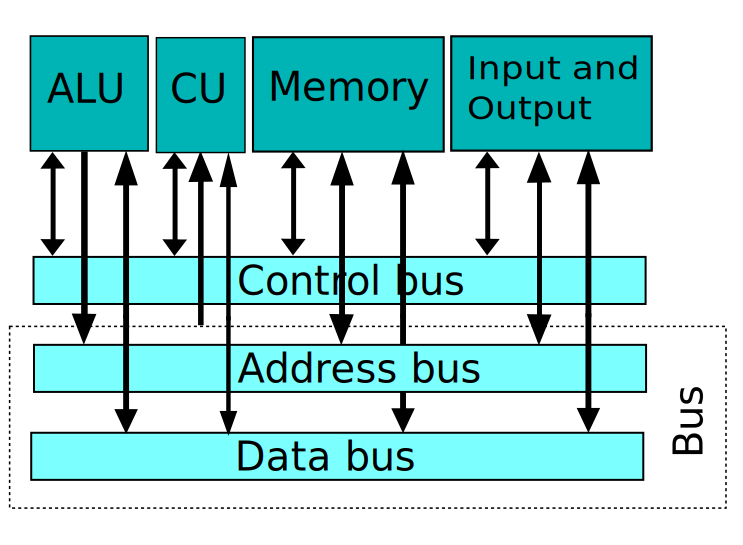
\includegraphics[width=0.5\textwidth]{figures/VNA}
  \end{center}
  \caption{The Von Neumann Architecture. Adapted from \cite{fig-vna}}\label{fig:vna}
\end{figure}

For this project, the data bus shall be referred to instead as the \textit{operand bus}, as its primary purpose is carrying operands. The combined address and operand bus shall be referred to as \textit{data bus}.

\subsection{Instruction Hierarchy}
The control unit controls the computer based on a \textit{program}. Each program serves a distinct purpose, e.g. calculating a series of numbers. It consists of multiple \textit{macro instructions}, which in return consist of multiple \textit{micro instructions}. Macro instructions perform, aligned with the von Neumann Architecture, an operation on a single \textit{data word}, such as overwriting it, or storing it somewhere else. A Micro instructions refers to the state of all control signals, e.g. if a component is reading or writing to the bus. Although it is possible to program a computer solely with micro instructions, it would be extremely inefficient, as the program code would be strongly repetitive \cite{malvino1983a}.

A collection of macro instructions is referred to as an \textit{instruction set}. 

\section{Tools} \label{sec:tools}

The most popular flavour of such a \textit{hardware description language} is Verilog, as defined in \textit{IEEE Std 1800-2023} \cite{10458102} and its extensions. Given widespread professional use of Verilog, more specifically the Verilog superset SystemVerilog, seemed to be the best option for this project as a large amount of information and guides on the topic exist. The terms SystemVerilog and Verilog will be used interchangeably. 

As the IEEE Standard only defines the language's syntax, a Verilog tool suite is required. Although previous experience in the usage of Verilog exists, expertise on the intricacies of Verilog simulation is still limited. It was thus decided based on the integration with other tooling, as to which suite is to be used. 

The key feature of the chosen suite, which is called \textit{Verilator}, is the compilation of the Verilog code to a binary and the generation of an interface to C++. Having an interface to C++ enables much more complex behaviours to be modelled in a simpler manner, such as reading test data from a file. Additionally, apart from being able to rely on previous experience in C++, it also allows me to make use of a vast ecosystem of testing, code coverage and development operations frameworks. Furthermore, the suite is available under the LGPL licence, allowing me to use it free of charge. I chose the GoogleTest framework for automated testing procedures. Most testing frameworks in essence do the same thing, although there are small nuances that differ from one to the other. 

Verilator also provides interfaces to coverage analysis tools by generating \textit{dumpfiles}. Dumpfiles contain the data of all signal values in the simulation across time and can be read by "digital oscilloscopes" like GTKWave. These can then be used to debug and understand the simulation, in case errors exist \cite{verilatoroverview}.

Git and GitLab are used as the version control system and development operations platform.

\subsection{Verilog Crash Course}
This section is not intended to be an exhaustive guide to Verilog, but only highlights the most important features and concepts relevant for this project. It is based on an internet guide \cite{verilogcourse}.

What differentiates simulated Verilog from other computer languages is its non-linear execution and its lack of a main function. Verilog files are not necessarily executed from top to bottom, but execution is based on propagation of signals throughout the interconnected modules. 

A module is declared with the \texttt{module} keyword. To complete a declaration the module must be named and ports specified. Ports are the connections going in and out of a module. They can either be an \texttt{input}, an \texttt{output} or bidirectional, denoted by \texttt{inout}. Ports are then specified like any other variable, by specifying the data type, length and name. For this paper usage of data types shall be limited to, \texttt{wire}, \texttt{reg}, \texttt{bit}, \texttt{logic} and for readability reasons \texttt{enum}. After the declaration of the ports the body of the module is defined, which contains the module logic.

\begin{lstlisting}[language=Verilog, caption=Module definition]
module <module_name> (
  input wire <input_name>,
  output reg <output_name>
);
<module_body>
endmodule
\end{lstlisting}


Most digital circuits are based around a clock signal and thus have to execute operations at every clock cycle. Verilog provides a way to model this with \texttt{always} blocks. Once the condition in the bracket is met, the code block is executed. Apart from simple boolean conditions, the block can also be executed at the rising and falling edge of a signal by using the \texttt{posedge} and \texttt{negedge} keywords.

\begin{lstlisting}[language=Verilog, caption=Always block definition]
always @(<condition>) begin
  <always_body>
end

\end{lstlisting}

As for the logic, the Verilog standard specifies if-blocks, loops, case statements and various logic and arithmetic operators comparable to other computer or programming languages. Unlike other languages, there are multiple types of assignments in Verilog. The easiest to understand is the continuous assignment with the \texttt{assign} keyword. This continuously assigns the value of the right-hand side to the left-hand side comparable to physical wires being connected together through logic gates. If the input changes, the output will change with it nearly instantaneously. The blocking assignment, denoted by the \texttt{=} operator, is used to assign values to variables instantaneously, like in other programming languages. The non-blocking assignment, denoted by the \texttt{<=} operator, only actually assigns the value to the left-hand side once the timing step, so every calculation in the current time step, is finished. 


The SystemVerilog standard also specifies a number of additional functions that are not synthesizable, so cannot be translated into hardware, but are useful for simulation, such as \texttt{\$display} and \texttt{\$finish}. As they are not synthesizable, they shall not be used, for this project. These features can be handled by the \texttt{C++} testbenches.



\subsection{Development Environment}
To reproduce the development environment for this project, the following packages need to be available in \texttt{PATH}. I suggest to use Debian 12. 

\begin{itemize}
  \item verilator@5.24
  \item a C++ tool chain (e.g. GCC)
  \item CMake
  \item a CMake generator (e.g. ninja)
\end{itemize}  

\begin{lstlisting}[caption=Build instruction, language=bash, label=lst:build]
# Make a new folder in the source directory
mkdir build
cd build
# Initalize CMake with the chosen generator. Here: ninja
cmake .. -GNinja
# Execute it
ninja

# To perfrom the tests execute ctest.
ctest

# To generate coverage info execute verilator_coverage
verilator_coverage -write-info logs/merged.info logs/*.dat

# Run gcov to produce a visual report
genhtml logs/merged.info --output-directory logs/html

# Open report
open logs/html/index.html
\end{lstlisting}

\section{Idea and Goal} \label{sec:goals}  
The following list can be understood as the top level requirements to this project:
\begin{itemize}
  \item Have a functioning computer architecture that:
 \begin{enumerate}
    \item Has an 8-bit bus width
    \item Is Turing equivalent
    \item Is based on the von Neumann Architecture
    \item Implements features wanted by me
    \item Is kept as simple as possible
  \end{enumerate}
  \item Have a simulation of this computer architecture that: 
  \begin{enumerate}
    \item Is fully tested, ensuring all requirements are met
    \item Is kept as simple as possible
    \item Can be interacted with by a user
    \item Is programmable by a higher level language (assembly)
  \end{enumerate}
\end{itemize}

Input and output capabilities are not intended to be developed, for this project, testbenches shall handle this.

Features that are wanted by me are intended to increase the feature set of the architecture to make it more useable and may or may not be based on my subjectivity. As such they shall not be evaluated.

Additionally, the process shall occur in a traceable manner, that is aligned to the process described in \ref{sec:chip-design}.

Implementation and execution of these goals shall be analysed in chapter \ref{chap:conclusion}.

\chapter{Designing the Architecture} \label{chap:arch}

This chapter treats the process steps of system specification and architectural design, with initial steps in logic design, as described in section \ref{sec:chip-design}.

Given the previously defined goals in section \ref{sec:goals}, three distinct groups of requirements to the computer architecture can be differentiated. Requirements resulting from the need for Turing equivalence are from here on out referred to as "Turing requirements".

Architectural requirements are a set of non-functional requirements given by the intended computer architecture. They are by design only verifiable and not testable.

Finally, feature requirements are requirements that are arbitrarily defined by me to expand the feature set. These requirements shall be justified, when put in place and tested.

Requirements are inlined and numbered to provide a point of reference to the text when implementing and testing them in the simulation. 

\newtheorem{turing-requirement}{Turing Req.}[section]
\newtheorem{arch-requirement}{Arch. Req.}[section]
\newtheorem{feat-requirement}{Feat. Req.}[section]

The keywords "must", "must not", "required", "shall", "shall not", "should", "should not", "recommended",  "may", and "optional" in the requirements are to be interpreted as described in RFC 2119 \cite{rfc2119}.



Following The Von Neumann the architecture shall be structured in a number of modules, the arithmetic logic unit, the control unit, memory, input and output. The modules interact with each over the three buses, sharing data, address and control signals. All actions are orchestrated by the control unit, signalling the other modules when to read or write data, when to perform calculations, and when to output data, based on the micro instructions stored in the control unit.

When taking into account that (random access) memory retrieval takes significantly longer than any other operation the von Neumann bottleneck can be alleviated to a certain extent by introducing a secondary, faster, form of memory. Deviating from the von Neumann Architecture the memory module shall be split up into to two modules, a random access memory, storing data and instructions referenced by addresses and the registers, storing only a single bus width (a data word). As well as a number of registers, storing operand data for the arithmetic logic unit. The registers function without an address and are directly operated by the control unit.

The modules, in which this architecture is split up to, thus are the arithmetic logic unit, the control unit, the memory, the register
and the input and output.
\begin{figure}[H]
  \begin{center}
    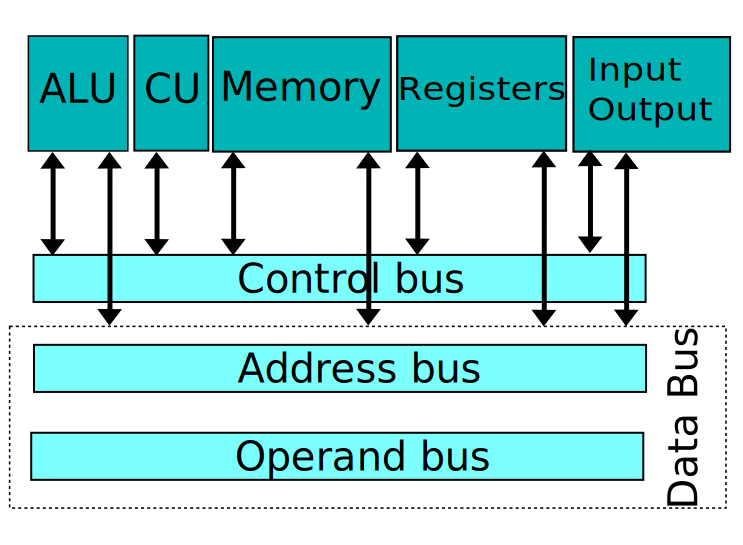
\includegraphics[width=0.5\textwidth]{figures/VNA-Adapted}
  \end{center}
  \caption{The Von Neumann Architecture. Adapted from \cite{fig-vna}}\label{fig:vna-adapted}
\end{figure}

\section{Arithmetic Logic Unit}
The Arithmetic Logic Unit is the module performing all arithmetic and logical operations on operands. It
is the centrepiece of the computer, as it is the only module that modifies, or synthesizes, new data.

The most commonly used and implemented arithmetic operation is addition and thus shall be the first operation to be implemented.
\begin{turing-requirement}
  Ability to add two data words.
\end{turing-requirement}

To source ideas for additional features and operations ChatGPT \cite{chatgptalu} was harnessed to generate ideas. From a number of suggestions, I decided to implement subtraction, shift, rotation and bit shift operations.

It additionally suggested features such as floating point maths, vector maths, multiplication and division. Multiplication and division however shall not be implemented, as these operations are not performable in a single iteration. Binary multiplication is normally achieved by repeated addition of the multiplicand to itself, whilst counting the addition operations, stopping when the multiplier is reached. The simplest way of performing a division, specifically integer division, is by repeated subtraction of the divisor from the dividend until a number smaller than the divisor is reached. As the architecture implements repeatable operations based on conditions, multiplication and division can be performed in macro code. This would be redundant. This also applies to any complex operations, such as vectors or logarithms; these will not be implemented.

Likewise, rotation and shift operations shall only be implemented for a single bit, as any other shift or rotation can only be achieved by performing the shift multiple times or by having multiple shift and rotate circuits in series.
\begin{feat-requirement} \label{req:sub}
  Ability to subtract two data words.
\end{feat-requirement}

\begin{feat-requirement}
  Ability to shift a data word bitwise.
\end{feat-requirement}

\begin{feat-requirement}
  Ability to rotate a data word bitwise.
\end{feat-requirement}

\begin{feat-requirement}
  Ability to AND, OR and XOR two data words.
\end{feat-requirement}

\begin{feat-requirement} \label{req:not}
  Ability to NOT a data word.
\end{feat-requirement}

Furthermore, the computer is required to be able to execute conditionally, thus requiring a condition. The indication of whether of this condition is true or not is called a flag. The two most common flags are the zero flag and the carry flag, as they can be easily generated mathematically. 

The carry flag, which indicates whether an addition in the ALU has overflown, so resulted in a number which is larger than the 8-bit data word size. Apart from being useful in conditional jumps, the carry flag can also be used to detect if a calculation has overflown, and thus if the result is incorrect.

\begin{turing-requirement}
  Generation of a carry flag. 
\end{turing-requirement}

The zero flag indicates if the result of an operation is zero. This is not only useful for looping a fixed number of times, but also for comparing two data words. As the ALU is designed to subtract two data words, a zero flag also allows for easy determination if two data words are equal, by subtracting them from each other. 

\begin{feat-requirement}
  Generation of a zero flag.
\end{feat-requirement}

Given the fact that the architecture has an 8-bit data bus and the arithmetic logic unit performs 8-bit operations, it will always need to buffer the two operands. Instead of having the ALU buffer the operands with two additional registers. It shall access two registers directly, that are otherwise, independent of the ALU.

\begin{arch-requirement}
  Ability to take in data from two registers.
\end{arch-requirement}

As the calculation results need to return to registers and memory, the ALU must have the ability to output data to the bus.
\begin{arch-requirement}
  Ability to output operation results to the bus. 
\end{arch-requirement}

Finally, the ALU shall not exert undefined behaviour in case of undefined control signals, and shall not output unless control signals indicate to do so. 


\begin{feat-requirement} \label{req:alu-no-output}
  Must not output unless control signals indicated to do so. 
\end{feat-requirement}
\pagebreak
\section{Memory}

\begin{turing-requirement}
Must allow writing to and reading from a memory location
\end{turing-requirement}

As instructions need data to operate on, the data, operands, and instructions should ideally be stored in a way that allows accessing one together with the other. The simplest approach would be to transfer the instruction together with the operand on to the bus, as in the SAP-2 architecture \cite{malvino1983a}.

Given that the 8-bit bus width is required, equally splitting the bus into four bits for the instruction and four bits for the operand would be the most straightforward approach.

This however results in only 16 possible instructions and the highest possible operand value of 15. Although this would not impact Turing completeness or any other requirement, it does not allow for an easily usable instruction set. In fact, manual programming of any "complex" task would be very difficult. One could achieve higher instruction count by reserving one instruction for all non-operand instructions and then using the last 4 bits to identify the individual instruction. This would allow for 31 instructions, 15 of which with operands up to 15.

Increasing the size of the instruction or operand is no option either as the other component would need to shrink, resulting in the architecture either having less instructions or smaller operands.

A solution to this problem is the introduction of a second data word that is stored in memory alongside, essentially increasing the address bus width by one. But instead of running this wire as part of the control bus. The indication of which data word is thus tied to the instruction's microprogramming and is not intended to be chosen at runtime. Additionally, this way of increasing the address bus does not require running a wire to every component, keeping the physical layout simple. Finally, the size of the stored program is also smaller, as the indication of the used data word is only stored once in the microcode contrary to repetitively storing it in the program code.  

As the selected data word must be configured per micro instruction in microcode before computer execution. Each data word is assigned a purpose. The first one storing the instruction and the second storing the operand.    

\begin{feat-requirement}
Must store, for each memory address, store two data words. A control signal shall indicate which data word to access. The first data word shall be intended for instructions and the second for operands.
\end{feat-requirement}

While an eight bit operand is considered sufficient for this architecture a program with only 255 instruction steps is not. Furthermore, to make the architecture Turing complete the architecture needs to be able to address infinite memory. To realize this, the primary addressing mode shall be relative. Additionally, the address width of the memory shall be extendable beyond the width of the 8-bit bus.

\begin{feat-requirement}
Must retrieve data with a relative memory address. 
\end{feat-requirement}

To allow for relative addressing, the program counter must be stored in full length. Additionally, to allow useful programming a second general purpose memory address register shall be implemented. % TODO: Explain better

\begin{feat-requirement}
Must store the program counter and memory address register.
\end{feat-requirement}

For certain features, such as a call stack, it is nonetheless useful to allow for absolute addressing. Additionally, first 8-bit of the program counter and memory address register shall be over writeable for absolute access.

\begin{feat-requirement}
Must retrieve data with an absolute memory address. 
\end{feat-requirement}


When the program is executed the first micro instruction will always be to increment the program counter to get the next instruction. As that "1" cannot come from the bus, as no instruction or memory is present for the first steps, the program counter must be able to be incremented without the bus.
\begin{feat-requirement}
    Must be able to increment the program counter by one with a specific control signal.
\end{feat-requirement}

\iffalse
With relative jumps of only 255 but bigger word counts. 
Assembler could impl like jump over 

PSEUDO
NORMAL PROGRAM
JMP2
JPD 255 
NORMAL PROGRAM RESUMES HERE
.
.
.
SOME OTHER PROGRAM THAT NEEDS TO JUMP MORE THAN ONE

\fi

\section{Registers}
As established in the architecture, the computer shall have a set of registers to store data words. The registers shall be able to store data words and output them to the bus.

\begin{feat-requirement}
  Ability to load a data word for storage.
\end{feat-requirement}

\begin{feat-requirement}
  Ability to output a data word.
\end{feat-requirement}

The registers that directly interface with the arithmetic logic unit must provide direct access to the register content without any control signals. 

\begin{arch-requirement} \label{req:register-direct-access}
  Must be able to be read by the ALU without any control signals.
\end{arch-requirement}


\section{Control Unit}
Following the von Neumann Architecture, the module orchestrating the interaction and operation of all modules is called the Control Unit. It is responsible for the generation of the control word, based on the macro program, the current state of the computer and current timing information. 

For every given combination of input the control word must produce a specific output forming a truth table. In historic computer architectures this truth table was represented by carefully creating a net of logic gates, which would produce the correct output for every input, to satisfy the truth table. 

With the increasing complexity and the fact that once physically produced this control logic could not be changed, the concept of the microcode was invented \cite{malvino1983a}. A storage, given enough address and data bus width, can represent any truth table, just like a combination of logic gates, with the key advantage of being reprogrammable. Thus, nowadays, control units are often not more than a piece of storage and a timing unit. If a silicon design is not intended to be micro-(re)-programmable, the storage/truth table can be minimized with certain algorithms and then hardwired into the silicon. As representing the truth table in a storage is the most flexible way, the control unit shall be implemented as a microcode storage.
\begin{arch-requirement}
  The microcode shall be implemented as storage.
\end{arch-requirement}

\begin{arch-requirement} \label{req:cw-from-instr}
  Must produce the control word (micro instruction) from instruction and state.
\end{arch-requirement}

To achieve Turing completeness, the control unit must be able to handle conditional operations based on flags.

\begin{turing-requirement}
  Must produce the control word from flags.
\end{turing-requirement}



\begin{arch-requirement}
  Must produce the clock signal. 
\end{arch-requirement}

Each clock cycle shall be counted to produce the \textit{timing state} count. A timing state is the time frame in which one micro instruction is executed. The number of timing states is determined by the number of micro instructions needed to execute an instruction. The number of required timing states, so the amount of micro instructions comprising one macro instruction, can only be determined once the exact instruction set is defined. Thus, the space needed in the control word for the timing state can only be estimated for now. Analysing the seemingly most complex instruction, a jump instruction, is a good starting point.
The required states for a basic jump instruction are: 
\begin{enumerate}
  \item Increment PC
  \item Fetch instruction (for certain jumps, only if the flags are set correctly)
  \item Fetch second data word (instruction argument) and increment program counter by it.
  \item Fetch instruction from new program counter
  \item Execute the new instruction
\end{enumerate}
    
As the execution of the newly targeted instruction will most likely take more than one step, the total count of timing states is thus is 6-8. Given that the timing state is represented in binary, the smallest number of bits needed to represent 8 states is 3. However, to ensure that the control unit could be used for more complex instructions, the number of timing states shall be set to 16 (4 bits).

\begin{arch-requirement}
  Must count clock cycles to produce 16 timing states and reset to zero once 16 was reached or the control word indicated to do so.
\end{arch-requirement}

To compensate for any redundant timing states a microcode signal to break out of the current instruction and skip to the next one is needed. 

\begin{feat-requirement}
  Must, given a specific output of the microcode break out of the current instruction (reset state signal).
\end{feat-requirement}


Given that for the computer to function every instruction must be first pointed to by the program counter and then loaded into the control unit, the relevant control words must be setup in the microcode. Instead of hard coding this into the control unit this shall be part of the standard microcode generation process.
\begin{feat-requirement}
  The control word generated by the first state, regardless of flag and macro instruction, must always increment the program counter by one. 
\end{feat-requirement}

\begin{feat-requirement}
  The control word generated by the second state, regardless of flag and macro instruction, must always fetch the current instruction and store it in the macro instruction register.
\end{feat-requirement}


\begin{feat-requirement}
  Must halt given micro/macrocode instruction to do so. 
\end{feat-requirement}

\section{Input and Output}
This architecture shall not specifically implement any input and output capabilities, as they are not required as per \ref{sec:goals}. Any input or output can be handled by testbenches, either by storing directly into memory cells or into registers.
\chapter{Implementing the Simulation}

\section{Development Operations }
Implementation of the DevOps was realised by leveraging the version control system (git) and the GitLab CI/CD platform. Replicating the local environmenta, a Debian based docker container \cite{dockerVerilator} was used in the pipelines. The pipelines is also set up to report code coverage and test results to the version control system platform for easy reference

As the version control system infrastructure does not provide any infrastructure to execute these pipelines, e.g. servers to run the docker containers, seperate machines were put in place and configured.



\section{Build System}
Verilator transforms the Verilog code into a binary and header files to address this binary. This, together with the testbench must be compiled into an executable. A google search of "Verilator GoogleTest" led to a repository containing a demostration for a SystemVerilog, Verilator and GoogleTest toolchain \cite{toolchain}. Luckily this is the exact combination of tools I want to use. 

GNU Make is used to first execute Verilator on all targets, which are defineable in the Makefile. The Makefiles which are generated by Verilator during \textit{verilation} are then set as additional Make targets and the corresponding testbench file is included.

Small adaptions of this buildchain were necessary to make it fit this project. Another folder of Verilog code, the \texttt{package} folder, must be always included, so that packages, in this project containing all enum definitionsm, can be used in the modules. Instead of passing only the Verilog files that are necessary, the build system now passes all source files and sets which module is the highest in the module hierarchy. 

Some flags that allow for Verilators timing and debugging features also have to be enabled.

The testbench example can be used, after adapting all necessary class names for all modules that do not generate, but only use the clock signal. The testbench 
for when Verilator needs to handle time, because a clock signal is generated, will be detailed later.

\section{Arithmetic Logic Unit}
Following the von Neumann Architecture all components recieve (and send) control signals, and are connected to the bus. 

There are two options for the ALU recieving the control signal indicating which operation to perform. Either each operation is represented by a single control signal or each operation is assigned a binary representation and then decoded in the ALU. The first approach would conform more to the VNA as all decoding would be performed in the control Unit, whereas with the second approach, the instruction would only fully be decoded in the ALU. The second approach is however much more efficient and readable. The first approach would require a 10 bit control signal whereas the second approach would only require $ceil(\log_2 10) = 4$ bits. Additionally the operations could be represented easily as an enumeration in Verilog ensuring readability. At first the first option was implemented and tested, but I decided to switch to the second option, because readability was not given. 

The two registers A and B are connected to the ALU directly, to conform with Arch. Req. 2.1.1. To implement testcases, the names of all signals must first be set and a module definition with these ports created, so that the testcases can be written.

\begin{table}[H]
\begin{tabular}{cccc}
  Type& Name & Purpose & \texttt{name}\\ \hline
  I   & Clock & Timing & \texttt{clock}\\
  O   & Bus     & Data output & \texttt{out}        \\
  I   & Register A and B & Data input & \texttt{register1} and \texttt{register2} \\
  I   & ALU control word & Control & \texttt{alu\_op\_e}\\
O   & Flag word & Control & \texttt{alu\_flag\_e}
\end{tabular}
\caption{ALU port list}
\label{tab:alu-i/o}
\end{table}

The implementation of the testcases for the ALU is straightforward for all requirements specifying an arithmetic or logic operation. Generally two arbitrary values are loaded into the registers and the correct control signals are sent to the ALU the clock cycled and then checked if the output is correct. 


\begin{lstlisting}[language=c++]
alu_dut->register1 = 1; 
alu_dut->register2 = 2; // The two registers are initalized with arbitrary values

alu_dut->op = alu::control::alu_op_e::ADD; // The control signal to add the two registers is set 

AdvanceClock();  // Clock is advanced, so that the operation is performed

EXPECT_EQ(alu_dut->result, 3); // Check if the result of the operation is correct.
\end{lstlisting}

The same applies to the tests for flag generation. Values are loaded to produce either of the flags and then it is tested if the flags are correctly generated.

The test case for Feat. Req. \ref{req:alu-no-output} is implemented by assigning arbitrary values and performing an operation without however enabling the output signal, finally checking if any data was latched onto the bus.  

Finally, the Verilog body of the module was based around a single \texttt{always\_ff} block. A switch case executes the correct operation based on \texttt{alu\_flag\_e}. The zero flag is generated by a continous assignment. The carry flag is generated by left padding the addition by one bit, removing the padding before latching the data onto the bus. The flags are latched into a register whenever an operation is performed, such that they are presistent until the next operation.

\section{Memory}

Following the principle of the ALU the memorys opcode is an enum. Apart from the control signal for the operation, the memory module requires additional control signals: the data word selector and address register selector.

All operations, except for absolute memory access requires an indication of which address register, PC or MAR, to use. The read and write operations additionally require the indication of the data word. 

\begin{table}[H]

  \centering
\begin{tabular}{cccc}
 Type & Name               & Datatype                       & name                          \\ \hline
 I    & Bus input          & \texttt{bit{[}7:0{]}}          & \texttt{input}                \\
 O    & Bus output         & \texttt{bit{[}7:0{]}}          & \texttt{output}               \\
 I    & Operation          & \texttt{memory\_op\_e}         & \texttt{op}                   \\
 I    & Data Word Selector & \texttt{bit}                   & \texttt{data\_word\_selector} \\
 I    & Address Register Selector       & \texttt{address\_register\_selector\_e} & \texttt{address\_register\_selector}        \\
 I    & Clock              & \texttt{bit}                   & \texttt{clock}               
 \end{tabular}

 \caption{Memory port list}
 \label{tab:memory-io}
\end{table}

For all tests, involving read operations, a value must be stored directly into the array that represents the physical memory cells in the simulation, this variable must also be defined already. To verify correct calculation of the different address modes the two address registers must also be defined. 

\begin{table}[H]
  \begin{center}
\begin{tabular}{ccc}
    Name               & Datatype                       & name                          \\ \hline
    Cells              & \texttt{bit{[}7:0{]} {[}1-ADDR\_BUS\_WIDTH+1{]}-1} & \texttt{cells} \\
    MAR                & \texttt{bit{[}(ADDR\_BUS \_WIDTH-1:0{]}} & \texttt{memory\_address\_register} \\
    PC                & \texttt{bit{[}(ADDR\_BUS\_WIDTH-1:0{]}} & \texttt{program\_counter} \\
    \end{tabular}
  \end{center}
    \caption{Memory internal net list}
    \label{tab:memory-internal-nets}

    
   \end{table}
   

Once again with the port and net list the test cases for the memory module are implemented. For the read operations and then the correct address is either loaded directly (absolute reads) or is the result of several operations (relative reads) where the address must first be calculated. For write operations the address is also either loaded directly or composed of multiple operations. The value that is to be wrriten is written onto the bus and the write operation is performed. The array is then checked at the address to see if the value is correctly written.

The read and write operations are implemented by reading/writing to the cells array with the index being the selected address register with the data word selector being appended as the least significant bit. The selected address bus is generated by a continous assignment based on the control signals. 

When specified, the value from the memory cells at the address specified by the selected bus and data word selector is latched onto the bus. When specified, the value on the input bus is written to the memory cells at the address specified by the selected bus and data word selector. They are thus executed in to seperate \texttt{always\_ff} blocks.

As continous assignments are used for the selected address bus, operations on the address registers cannot be done on the selected address bus variable. Instead the address registers are modified directly with an \texttt{if} statement.


\section{Register}
The register will is implemented in two seperate modules, one complying with all requirements, the second one without \ref{req:register-direct-access} direct access for the alu. As they are four registers and only two are connected to the ALU, having direct access present in the other two would be redundant. The register implementing the direct access is named \texttt{reg\_acc}, the other \texttt{reg\_tmp}.

The register module is the simplest of all modules. Only bus input and output, clock and a control signal are required. The bus is connected as input and output.

\begin{table}[H]
  
  \begin{center}
  \begin{tabular}{cccc}
   Type & Name               & Datatype                       & name                          \\ \hline
   I    & Bus input          & \texttt{bit{[}7:0{]}}          & \texttt{input}                \\
   O    & Bus output         & \texttt{bit{[}7:0{]}}          & \texttt{output}               \\
   I    & Operation          & \texttt{reg\_op\_e}         & \texttt{op}                   \\
   I    & Clock              & \texttt{bit}                   & \texttt{clock}               \\
   O    & ALU Direct Access               & \texttt{bit{[}7:0{]}}          & \texttt{reg\_direct}               \\
   \end{tabular}
  \end{center}
   \caption{Register port list}
   \label{tab:reg-io}
\end{table}

The last entry is only present in the \texttt{reg\_acc} module. The test cases for the register module are implemented similarly to those for the ALU and memory. 

For both modules, the module is split into two \texttt{always\_ff} blocks, one for reading and one for writing. The reading block is executed on the rising edge of the clock signal and the writing block on the falling edge. The reading block is a simple assignment of the output to the input. The writing block is a simple assignment of the input to the output. The direct access is implemented by a continous assignment.


\section{Control Unit}
The Control Units port list can be derived from all the signals that are required on the other modules. 

\begin{table}[H]
  
  \begin{center}
  \begin{tabular}{cccc}
   Type & Name               & Datatype                       & name                          \\ \hline
   I    & Bus input          & \texttt{bit{[}7:0{]}}          & \texttt{input}                \\
   O    & Clock              & \texttt{bit}                   & \texttt{clock}               \\
   O    & Memory Operation   & \texttt{memory\_op\_e}         & \texttt{memory\_op}           \\
   I    & ALU flag          & \texttt{alu\_flag\_e}          & \texttt{alu\_flag}            \\
   O    & ALU control word & \texttt{alu\_op\_e}         & \texttt{alu\_op}                   \\
   I    & 4x Reg Operation   & \texttt{reg\_op\_e}         & \texttt{r\*x\_op}                   \\
    \end{tabular}
  \end{center}
   \caption{Control Unit port list}
   \label{tab:reg-net-list}
\end{table}

To implement testcases for the control unit additonal variabls internal to the control unit must be defined. To test generation of timing information, the timing state count variable must be defined. The test cases for microcode generation must have access to the microcode storage.

\begin{table}[H]
  \begin{center}
  \begin{tabular}{ccc}
    Name               & Datatype                       & name                          \\ \hline
    Timing state count & \texttt{bit{[}3:0{]}}          & \texttt{state}                \\
    Microcode          & \texttt{bit{[}(\`CW\_WIDTH\-1):0{]} {[}(1$<<$MIW\_WIDTH)\-1{]}} & \texttt{microcode}                \\
  \end{tabular}

\end{center}
  \caption{Control Unit internal variables that are required for testing}
   \label{tab:reg-io}

  \end{table}

All test related to timing are implemented by advancing time in the simulator and observing clock and timing state behaviour, including the state rolling over to zero. The test cases for microcode generation are implemented by loading single control words, generated by a helper library, into the microcode storage at address that are expected, then advancing time and checking if the correct control word is output and if all parts of the control word, generated by the helper library, are output to the correct output signals. 

At every rising edge of the clock signal, the state is counted up, rolling back to 0 once the maximum number of states was reached or the control signal for the next instruction is high.


The microcode is read and written out to the control word at the falling edge of the clock. 

\section{Build system switch}
The original build system turned out to be extremely limited as soon as additional libraries needed to be included. I thus decided to switch away from Make to CMake because I had previous experience with it.

As the build system is not necessarily part of the product, EXPAND, I decided to employ ChatGPT to write the new build system. At first, ChatGPT incorrecctly used Verilator inside of the CMake file, instead of using the Verilator plugin, it called Verilator as a binary. After providing it with Verilator's documentation, ChatGPT fixed the mistake and provided a functioning build system. 

Some additional modifications were made, to correctly include and fetch the GoogleTest library, such that it can be compiled against. 

The new build system does exactly the same as the old one apart from the allowing for easier inclusion and compilation of libraries. Instead of having to provide each indivdual C++ file to the make command, all files in the \texttt{lib} directory are now usable in the testbenches.

\section{Helper Libraries}
The simulation shall be programmable in assembly as per the goals of this project. The architecture, and the simulation for that matter, however are only directly programmable by macro instructions that are in return translated into micro instructions by the control unit. To bridge that gap, several libraries were introduced that make this possible. 

Together these libraries handle the process from instruction definitions and assembly code to microcode and macro programm. The whole process is logically split up into 7 libraries. All libraries implement a builder pattern. 

The process of reaching a functioning programm begins with the definition of the microcode handler. The microcode handler is then loaded with macro instructions. During the intalization of the microcode handler, the states to fetch and load the new instructions are already put into the microcode.

\begin{lstlisting}[caption=Inialization of the Microcode]
auto FibMicrocode = (new Microcode()); // Initalize the Microcode handler

FibMicrocode->AddMacroInstruction( 
    (new MacroInstruction("LDA")) // Initalize new macro instructions with name LDA. 
        ->set_next_state((new TimingState( // Set first start. 
            (new ControlWord()) 
                ->set_data_word_selector(1)
                ->set_memory_bus_selector(cpu_control::memory_bus_selector_e::PC)
                ->set_memory_op(cpu_control::memory_op_e::READ)
                ->set_rax_op(cpu_control::reg_op_e::LOAD))))); // Set control word bits.
\end{lstlisting}

The control word provided at construction of a \texttt{TimingState} is implicitly set for all possible flags. The \texttt{TimingState} class provides a method to overwrite a control word for a single flag. Jump instructions can harness this to only execute jumps if specific flags are set.

After adding all macro instructions, the microcode is computed. Each macro instruction is given an opcode, which is stored for later reference, remaining states filled with a control word that indicates jumping to the next instruction. Finally, all instructions are converted to binary and concatenated, to be stored in an instance of the simulation. 

To then program in assembly, an assembler must be created and supplied with the opcodes and instruction names. To reduce unncessary complexity by introducing a string parsing, this assembler does not use a classical assembly file but instead the program can be built step by step with a builder pattern. 
\begin{lstlisting}[caption=Inialization of Assembler and programming of macrocode ]
// The assembler is initalized and the Microcode passed to get opcodes
auto FibAssembler = new Assembler(FibMicrocode); 

FibAssembler->next("LDA", 0)->next("LDB", 1); // Add instructions with arguments
for (int i = 0; i < 10; i++) {
    // Add instructions to calculate fibonacci
    FibAssembler->next("ADD")->next("MBA")->next("MCB"); 
}
FibAssembler->next("HLT"); // Finally halt the computer

// Assemble the code and copy into simulation instance.
FibAssembler->StoreIntoModel(cpu_dut->rootp->cpu__DOT__memory__DOT__cells.m_storage); 
\end{lstlisting}

At first, these libraries did not function correctly. Both binaries, microcode and macro program, were seemingly random. After some investigation, the root cause turned out to be unallocated memory. In an attempt to increase the readability I forgot allocating all of the different objects. During one late programming session I was under the impression that the allocation would be performed by the constructor and omitted the new. \texttt{ControlWord()->set\_data\_word\_selector()} is in fact much more readable, than\texttt{{new ControlWord()}->set\_data\_word\_selector()}, however sadly not functions correctly.

A test case was introduced, to ensure, that during programming of the helper libraries, no errors were introduced in the binary arithmetics for control word and microcode generation.

\section{Integration of all modules}
The integration of all modules is achieved by instantiaing all modules and connecting the ports. To test the integrated \texttt{CPU}, refered to as a \textit{unit}, whole macro programs are loaded. This was straightforward. 

After initial tests however, the computer did not function. During close analysis of the timing diagrams created during the tests, it became clear that the macro instruction was not correctly loaded into the instruction register in the control unit. 

\section{Timing Issues}
After the first instruction in the assembly is read from the memory at state 0x3, the load signal goes high, which should trigger a latch into the register, given the module code. 

\begin{lstlisting}[caption=Instruction Register Code]
always_ff @(negedge clock) begin
[...]
if (load) begin
  macro_instruction <= bus;
end
[...]
end
\end{lstlisting}

A timing diagram however clearly shows, that the register remains empty.
\begin{timingdiag}[!ht]
\begin{center}
\begin{tikztimingtable}
    clock              & L H L H L H \\ 
    load               & L L H H L L \\
    memory\_op          & 2L 2D{READ} 2L \\ 
    bus[7:0]           & 2D{00} 2D{01} 2D{00} \\
    macro\_instruction[7:0] & 6L \\ 
\end{tikztimingtable}
\end{center}
\caption{Execution of primer micro instructions.}
\end{timingdiag}


Revisiting the corresponding Verilog code, it indicated no reason, on why the latching into the register wouldn't function as long as there is data on the bus. After several tests and some research into assignments in Verilog, it became obvious that there was a architectural flaw in the implementation. But it was unclear where this flaw was. Moving focus from development onto the paper, the flaw immediately clear. As initally intended and written in early drafts of the paper, cf. Git commit 57c6dc669, content should be "Onto bus at rising clock, from bus at falling clock.". This was however never translated into a formal requirement, and thus forgotten during implementation. 

Up until now all operations the computer performed, apart from the control unit, were performed at the rising edge of the clock. This meant that during writing to the bus by one module, another already tried to read that data, but that data hadn't yet propagated to it, which lead to no data being read at all. To rectify this issue all read operations in modules, so control unit, memory, and registers, were moved out of the rising edge \texttt{always\_ff} block into a new \texttt{always\_ff}. 

\begin{arch-requirement} \label{req:bus-read-write}
  All writes to the bus must occur at the rising edge of the clock. All reads from the bus must occur at falling edge of the clock.
\end{arch-requirement}

After an additional bug fix in the microcode generation, where macro program code was overwriting the fetch control word in the final microcode, execution of simple programs was successful.


\section{Conceptional Issues with Jumps}
During development of the demonstration for \ref{sec:nth-sum} it became clear that jumps were not possible as initally intended. 

Jump instructions were intended to work by giving an instruction that has a specific condition in microcode and that has the instruction to jump to as an argument. Given the current implementation of the memory module this would not be possible, as the memory would need to receive two instructions concurrently. 

The first to output the argument, so the second data word, to the bus, the other to subtract or add this data word to program counter. To solve this concurrency issue, either the addressing module receives its own independent control signal, or the argument is instead of loaded with the jump instruction, stored in a register and accessed from there. 

Although the second option would result in a simpler module, and smaller control bus width, the resulting processing overhead would be enormous. As explained earlier memory reads are extremely time expensive and having to read the address offset every time even though it is maybe not needed, warrants this extra complexity.

To implement this change, modifications were needed in the control unit, adding another control signal, the memory module, implementing this second control word, by adding case statements and the helper libraries, so corresponding micro and macro code can be generated. During modification for this new feature it was also noticed that Arch. Req. \ref{req:bus-read-write} was improperly implemented in the memory module, where modifications to the address buses would be handled at rising edge, and not at falling edge. This was mistake was also corrected.

\section{Flag latching}
Further development of the demonstration for \ref{sec:nth-sum} made a mistake in the status flag implementation apparent. Up until now the status flags were generated by a continous assignment in the ALU, which depended on the enable signal of the ALU. This lead to the flags never being available to the control unit, as the continous assignment returned to zero after disabling the ALU. Moving this assignment to latch into the output register rectifies this problem.


\chapter{Functional Demonstration}
This chapter is intended to demonstrate the function of the computer as per defined in section \ref{goal} by running at first simple well known algorithms and finally demonstrating Turing equivalence by implementing a \textit{Brainfuck} interpreter. % Nope it wasn't chatgpt, it was THC.




\section{Fibonacci Sequence}
The Fibonacci sequence is a simple sequence of natural numbers, where an element in the sequence is given by the sum of the perceding two elements.

The required instructions for generating assembly are thus relatively simple. The only instructions required are those for moving data in and out of registers, initalizing them and adding them. A halt instruction is also added so that the simulation can stop when calculations are done. 

For this demonstration the calculations do not yet happen in a loop but the instructions are just repeated a number of times. Loops and conditions are intended to be demostrated in section \ref{sec:n-num}.

Creating the control words for the instructions is straight forward. For the load instructions, the memory is set to read the second data word, from the current instructions, either storing it into register A or register B. The move instructions set one of the registers to output and one to load. Finally the ADD instruction, activates the ALU, sets its operation to "ADD" and sets the C register to load. 

The final macro programm then looks like this: 
\begin{lstlisting}[language={[x86masm]Assembler}, caption=Assembly code to calculate assembly, label=lst:fib]
LDA 0 ; Initalize register A with 0
LDB 1 ; Initalize register B with 1
ADD ; Add register A and B and store into register C
MBA ; Move register B to A
MCB ; Move register C to B
... ; Repeat ADD, MBA, MCB n times to reach the (n+1)th element
HLT ; Signal execution is complete
\end{lstlisting}

After generating the microcode and macro program, the following content of the three used registers can be observed during the execution of the programm, assuming that the three instructions are repeated 10 times:

\begin{timingdiag}[!ht]
\begin{tikztimingtable}
    % clock               & 0.004L0.005H0.005L0.005H0.005L0.005H0.005L0.005H0.005L0.005H0.005L0.005H0.005L0.005H0.005L0.005H0.005L0.005H0.005L0.005H0.005L0.005H0.005L0.005H0.005L0.005H0.005L0.005H0.005L0.005H0.005L0.005H0.005L0.005H0.005L0.005H0.005L0.005H0.005L0.005H0.005L0.005H0.005L0.005H0.005L0.005H0.005L0.005H0.005L0.005H0.005L0.005H0.005L0.005H0.005L0.005H0.005L0.005H0.005L0.005H0.005L0.005H0.005L0.005H0.005L0.005H0.005L0.005H0.005L0.005H0.005L0.005H0.005L0.005H0.005L0.005H0.005L0.005H0.005L0.005H0.005L0.005H0.005L0.005H0.005L0.005H0.005L0.005H0.005L0.005H0.005L0.005H0.005L0.005H0.005L0.005H0.005L0.005H0.005L0.005H0.005L0.005H0.005L0.005H0.005L0.005H0.005L0.005H0.005L0.005H0.005L0.005H0.005L0.005H0.005L0.005H0.005L0.005H0.005L0.005H0.005L0.005H0.005L0.005H0.005L0.005H0.005L0.005H0.005L0.005H0.005L0.005H0.005L0.005H0.005L0.005H0.005L0.005H0.005L0.005H0.005L0.005H0.005L0.005H0.005L0.005H0.005L0.005H0.005L0.005H0.005L0.005H0.005L0.005H0.005L0.005H0.005L0.005H0.005L0.005H0.005L0.005H0.005L0.005H0.005L0.005H0.005L0.005H0.005L0.005H0.005L0.005H0.005L0.005H0.005L0.005H0.005L0.005H0.005L0.005H0.005L0.005H0.005L0.005H0.005L0.005H0.005L0.005H0.005L0.005H0.005L0.005H0.005L0.005H0.005L0.005H0.005L0.005H0.005L0.005H0.005L0.005H0.005L0.005H0.005L0.005H0.005L0.005H0.005L0.005H0.005L0.005H0.005L0.005H0.005L0.005H0.005L0.005H0.005L0.005H0.005L0.005H0.005L0.005H0.005L0.005H0.005L0.005H0.005L0.005H0.005L0.005H0.005L0.005H0.005L0.005H0.005L0.005H0.005L0.005H0.005L0.005H0.005L0.005H0.005L0.005H0.005L0.005H0.005L0.005H0.005L0.005H0.005L0.005H0.005L0.005H0.005L0.005H0.005L0.005H0.005L0.005H0.005L0.005H0.005L0.005H0.005L0.005H0.005L0.005H0.005L0.005H0.005L0.005H0.005L0.005H0.005L0.005H0.005L0.005H0.005L0.005H0.005L0.005H0.005L0.005H0.005L0.005H0.005L0.005H0.005L0.005H0.005L0.005H0.005L0.005H0.005L0.005H0.005L0.005H0.005L0.005H0.005L0.005H0.005L0.005H0.005L0.005H0.005L0.005H0.005L0.005H0.005L0.005H0.005L0.005H0.005L0.005H0.005L0.005H0.005L0.005H0.005L0.005H0.005L0.005H0.005L0.005H0.005L0.005H0.005L0.005H0.005L0.005H0.005L0.005H0.005L0.005H0.005L0.005H0.005L0.005H0.005L0.005H0.005L0.005H0.005L0.005H0.005L0.005H0.005L0.005H0.005L0.005H0.005L0.005H0.005L0.005H0.005L0.005H0.005L0.005H0.005L0.005H0.005L0.005H0.005L0.005H0.005L0.005H0.005L0.005H0.005L0.005H0.005L0.005H0.005L0.005H0.005L0.005H0.005L0.005H0.005L0.005H0.005L0.005H0.005L0.005H0.005L0.005H0.005L0.005H \\
    % state               & 0.08L0.2D{1}0.2D{2}0.2D{3}0.2D{4}0.2D{5}0.2L0.2D{1}0.2D{2}0.2D{3}0.2D{4}0.2D{5}0.2L0.2D{1}0.2D{2}0.2D{3}0.2D{4}0.2D{5}0.2L0.2D{1}0.2D{2}0.2D{3}0.2D{4}0.2D{5}0.2L0.2D{1}0.2D{2}0.2D{3}0.2D{4}0.2D{5}0.2L0.2D{1}0.2D{2}0.2D{3}0.2D{4}0.2D{5}0.2L0.2D{1}0.2D{2}0.2D{3}0.2D{4}0.2D{5}0.2L0.2D{1}0.2D{2}0.2D{3}0.2D{4}0.2D{5}0.2L0.2D{1}0.2D{2}0.2D{3}0.2D{4}0.2D{5}0.2L0.2D{1}0.2D{2}0.2D{3}0.2D{4}0.2D{5}0.2L0.2D{1}0.2D{2}0.2D{3}0.2D{4}0.2D{5}0.2L0.2D{1}0.2D{2}0.2D{3}0.2D{4}0.2D{5}0.2L0.2D{1}0.2D{2}0.2D{3}0.2D{4}0.2D{5}0.2L0.2D{1}0.2D{2}0.2D{3}0.2D{4}0.2D{5}0.2L0.2D{1}0.2D{2}0.2D{3}0.2D{4}0.2D{5}0.2L0.2D{1}0.2D{2}0.2D{3}0.2D{4}0.2D{5}0.2L0.2D{1}0.2D{2}0.2D{3}0.2D{4}0.2D{5}0.2L0.2D{1}0.2D{2}0.2D{3}0.2D{4}0.2D{5}0.2L0.2D{1}0.2D{2}0.2D{3}0.2D{4}0.2D{5}0.2L0.2D{1}0.2D{2}0.2D{3}0.2D{4}0.2D{5}0.2L0.2D{1}0.2D{2}0.2D{3}0.2D{4}0.2D{5}0.2L0.2D{1}0.2D{2}0.2D{3}0.2D{4}0.2D{5}0.2L0.2D{1}0.2D{2}0.2D{3}0.2D{4}0.2D{5}0.2L0.2D{1}0.2D{2}0.2D{3}0.2D{4}0.2D{5}0.2L0.2D{1}0.2D{2}0.2D{3}0.2D{4}0.2D{5}0.2L0.2D{1}0.2D{2}0.2D{3}0.2D{4}0.2D{5}0.2L0.2D{1}0.2D{2}0.2D{3}0.2D{4}0.2D{5}0.2L0.2D{1}0.2D{2}0.2D{3}0.2D{4}0.2D{5}0.2L0.2D{1}0.2D{2}0.2D{3}0.2D{4}0.2D{5}0.2L0.2D{1}0.2D{2}0.2D{3}0.2D{4}0.2D{5}0.2L0.2D{1}0.2D{2}0.2D{3}0.2D{4}0.2D{5}0.2L0.2D{1}0.2D{2}0.2D{3}0.2D{4}0.2D{5}0.2L0.2D{1}0.2D{2}0.2D{3}0.1D{4} \\
    macro\_instruction  & 0.58L1.2D{1}1.2D{2}1.2D{3}1.2D{4}1.2D{5}1.2D{3}1.2D{4}1.2D{5}1.2D{3}1.2D{4}1.2D{5}1.2D{3}1.2D{4}1.2D{5}1.2D{3}1.2D{4}1.2D{5}1.2D{3}1.2D{4}1.2D{5}1.2D{3}1.2D{4}1.2D{5}1.2D{3}1.2D{4}1.2D{5}1.2D{3}1.2D{4}1.2D{5}1.2D{3}1.2D{4}1.2D{5}0.2D{6} \\
    reg\_a              & 4.58L7.2D{1}3.6D{2}3.6D{3}3.6D{5}3.6D{8}3.6D{13}3.6D{21}3.6D{34}2.2D{55} \\
    reg\_b              & 2.18L7.2D{1}3.6D{2}3.6D{3}3.6D{5}3.6D{8}3.6D{13}3.6D{21}3.6D{34}3.6D{55}1.0D{89} \\
    reg\_c              & 3.38L3.6D{1}3.6D{2}3.6D{3}3.6D{5}3.6D{8}3.6D{13}3.6D{21}3.6D{34}3.6D{55}3.4D{89} \\
\end{tikztimingtable}
\caption{Execution of Listing \ref{lst:fib}. Signal names adapted for readability.}
\end{timingdiag}

Manually calculation of the $11$th element leads to the same result of $89$.

\section{Sum of first $n$ natural Numbers} \label{sec:nth-sum}
The goal of this demonstration is to show the functioning of the conditional operation and thus also looping. The program shall continously add the next natural number until the sum would be greater than 255 and thus the carry flag triggered. The following python code illustrates the approach and can be used to calculate the expected result.

\begin{lstlisting}[caption=Python code for the generation of the sequence]
sum = 0
num = 1
while (sum+num) < 255:
    sum += num
    num +=1
print(sum)
print(num)
\end{lstlisting}

Executing this script results in $253$ for the expected sum and $23$ as the result for the number of iterations. 

The assembly instructions required for this are limited to initializing the registers, adding and moving around as well as a jump instruction, that is only performed when the carry flag is not set. 

\begin{lstlisting}[caption=Assembly code for the generation of the sum of $n$ natural numbers below 255, label=lst:nsum]
LDB 0
LDC 0 ; Init the registers with 0
LDA 1 ; Load 1 into register A
ADB   ; Add registers A and B and store into B
MCA   ; Move register C into A
ADC   ; Add registers A and B and store into C
JNC 5 ; Jump four instructions backward if carry not set. 
; Jump is instructed to one beforehand so, it points to ADB after the increment
HLT   ; Halt computer
\end{lstlisting}

After configuring the microcode and assembler with these instructions, the sum, that is expected to be $253$ and the last summand $23$ can be observed in the timing diagrams generated during execution: 

\begin{timingdiag}[!ht]
\begin{tikztimingtable}
is\_carry & 55.552L0.84H \\
halt & 56.392LG \\
reg\_a & 1.352L0.96D{1}1.44L3.36D{1}1.44D{3}0.96D{1}1.44D{6}0.96D{1}1.44D{10}0.96D{1}1.44D{15}0.96D{1}1.44D{21}0.96D{1}1.44D{28}0.96D{1}1.44D{36}0.96D{1}1.44D{45}0.96D{1}1.44D{55}0.96D{1}1.44D{66}0.96D{1}1.44D{78}0.96D{1}1.44D{91}0.96D{1}1.44D{105}0.96D{1}1.44D{120}0.96D{1}1.44D{136}0.96D{1}1.44D{153}0.96D{1}1.44D{171}0.96D{1}1.44D{190}0.96D{1}1.44D{210}0.96D{1}1.44D{231}0.96D{1}1.28D{253} \\
reg\_b & 1.832L2.4D{1}2.4D{2}2.4D{3}2.4D{4}2.4D{5}2.4D{6}2.4D{7}2.4D{8}2.4D{9}2.4D{10}2.4D{11}2.4D{12}2.4D{13}2.4D{14}2.4D{15}2.4D{16}2.4D{17}2.4D{18}2.4D{19}2.4D{20}2.4D{21}2.4D{22}1.76D{23} \\
reg\_c & 2.792L2.4D{1}2.4D{3}2.4D{6}2.4D{10}2.4D{15}2.4D{21}2.4D{28}2.4D{36}2.4D{45}2.4D{55}2.4D{66}2.4D{78}2.4D{91}2.4D{105}2.4D{120}2.4D{136}2.4D{153}2.4D{171}2.4D{190}2.4D{210}2.4D{231}2.4D{253}0.8D{20} \\
\end{tikztimingtable}
\caption{Execution of Listing \ref{lst:nsum}. Signal names adapted for readability}
\end{timingdiag}



\section{Brainfuck}
Proving computational universality or Turing completeness can become very convoluted. The simplest way to prove it is to demonstrate Turing equivalence to a Turing machine, by simulating one. Directly simulating a Turing machine is a valid and feasible method to do so. However, Turing machines have the concept of "states" in which the machine can be. As this architectures' concept of states is limited complex additional logic would need to be programmed. A Turing complete language that is more easily interpretable by this architecture is \textit{Brainfuck}. Brainfuck is an esoteric language that generally consists only of six instructions for logic, and two for input and output. It is however not standardized by any governing authority, and thus has a vast number of inscrutable definitions, standards and extensions. Apart from not implementing the input and output instructions (\texttt{.} and \texttt{;}), deviating from, what seems to me the given standard, the loop is implemented as a \texttt{do-while} loop instead of a normal \texttt{while} loop. This significantly eases implementation, as the compiler or interpreter doesn't have to look ahead in the program, but only back. This has no impact on Turing equivalence. 

\begin{table}[H]
\begin{center}
\begin{tabular}{ccc}
Instruction    & Purpose                  & C++ equivalent                       \\ \hline
\texttt{+}             & Increment at the pointer & \texttt{ptr*++;}                   \\
\texttt{-}               & Decrement at the pointer & \texttt{ptr*--;}                   \\
\texttt{\textgreater{}} & Increment the pointer    & \texttt{ptr++;}                    \\
\texttt{\textless{}}   & Decrement the pointer    & \texttt{ptr--;}                    \\
\texttt{{[}}            & Begin loop               & \texttt{do \{}                     \\
\texttt{{]}}            & End loop              & \texttt{\} while(ptr*);}
\end{tabular}
\end{center}
\caption{Brainfuck instruction table}
\label{tab:brainfuck-instructions}
\end{table}

All instructions are logically split up in multiple macro instructions. Both \texttt{+} and \texttt{-} are structured the same way, first the content of the current cell is loaded into register A and register 2 is loaded with one. Then, depending on the instruction, either an addition or a subtraction is performed by the ALU and stored back into the current cell. For \texttt{\textgreater} and \texttt{\textless} a one is once again loaded into the B register and a relative addition or subtraction is preformed on the \texttt{memory\_address\_register}. For the \texttt{{[}} no macro instructions are set. Instead, the current instruction count is stored temporarily. Once the corresponding \texttt{{]}} is reached, the current memory cell is compared against zero. If the cell content is larger than zero a jump backwards is performed. The jump back is calculated with the previously stored instruction count and the current instruction count.

The following instruction set was thus developed:
\begin{table}[]
    \begin{centering}
    \begin{tabular}{cc}
    Instruction & Purpose                                                                  \\ \hline
    LDA         & Load value, pointed to by memory address register, into register A       \\
    LDB         & Load second data word into register B                                    \\
    ADS         & Add register A and B and store into current memory address               \\
    SUS         & Subtract register A and B and store into current memory address          \\
    REA         & Add to the memory address register, what is currently in register B      \\
    RES         & Subtract to the memory address register, what is currently in register B \\
    JNE         & Jump back if not equal, as much as register B specifies                  \\
    HLT         & Halt computer                                                           
    \end{tabular}
\end{centering}
    \caption{Brainfuck macro instruction set.}
    \label{tab:brainfuck-macro-instructions}
    \end{table}

Before any of the Brainfuck program is converted to these macro instructions. The memory address register is first moved away from zero, such that it does not interfere with the program code.

Finally, in a loop the macro instructions for the following program are computed: 

\begin{lstlisting}[caption=Brainfuck program, label=lst:brainfuck]
    ++>>+++++[-[-]]>>+++
\end{lstlisting}

This program first increments the first memory cell by two, then moves two to the right, and increments this by 5, and then preforms two loops. The outer loop only performs one subtraction, before another loop is started that is executed four times, such that the cell is zero, which also causes the second loop to exit. Finally, the pointer is incremented twice again and then the cell is incremented thrice. 

The test bench then checks if the first address is at zero, and if the fourth address is 3.

The program is written arbitrarily, has each instruction once, and has nested loops, to ensure, that nesting functions. 



\chapter{Conclusion} \label{chap:conclusion}
This chapter concludes this project by first evaluating the product and process based on the goals defined in \ref{sec:goals}.

\section{Evaluation}
The most important requirement to me, of having an 8-bit bus width is complied with. All data, be it operands or addresses always travels over eight bits at some point. The requirement of Turing equivalence to a Turing machine was demonstrated successfully by first demonstrating the ability to interpret Brainfuck, which is in return Turing complete.

Implementation of the von Neumann Architecture was done on best effort basis. Naming schemes and the applied modularization adhere to it. Deviations from it occurred by introducing registers. Registers as such do not follow von Neumann's idea of having a unified memory for instructions and operands. Nonetheless, the registers are considered essential.

Furthermore, the augmentation of the address bus is not considered to be a deviation from the von Neumann architecture. The intention behind the idea that all data (cf. section \ref{subsec:vna}) travels over the same bus is to ensure that the data and instructions can be stored in the same memory.

The requirement of a four bit timing state and its justification have been disproved by the demonstrations in section \ref{chap:demo}. None of the instructions have more than one state. Although there exists optimization potential for some instructions, by combining them, none of them would come close to the maximum of 16. The provided jump example lost its validity, by simply jumping one more or less instruction, such that execution of the target instruction can be achieved by normal execution flow (e.g. increment of program counter and loading of instruction into control unit). A reduction of timing states to three or even two bits would be valid.

Analysing the simulation, the generated coverage report (report generation cf. section \ref{lst:build}) indicates that only $52.6\%$ of the code is covered. Many of the supposedly uncovered lines, are however clearly covered. For example, all operations apart from the addition are reported to be untested, however the tests for requirements \ref{req:sub} to \ref{req:not} clearly test these operations (cf. \texttt{alu\_test.cpp}). This test report is thus considered to be faulty and disregarded. A test report that is only based on tests from modules and not on entire \texttt{CPU} tests shows a coverage of $98.5\%$.

At a total number of 137 lines of code, this leaves only two lines uncovered. These two lines are a port definition and a line concerning macro instruction decoding. Interesting enough, these lines of code are not explicitly covered by any requirements. The only requirement defining it, is \ref{req:cw-from-instr}. It only states, that control word must be generated from flags. The simulation now however also implements a register to store the current macro instruction, such that the instruction can be decoded over several steps. A feature essential to the operation of the simulation. 

This coincides with the errors that were discovered and rectified in sections \ref{sec:timing-issues} through \ref{sec:flag-latching}. These problems all can be traced back to the first design steps, where either a requirement was not broken down enough or the exact behaviour was never specified. This is confirmed by the fact that before programming for section \ref{chap:demo}, so after section \ref{sec:integration} the entire test suite for individual components passed.

\section{Reflection}
This inevitably leads to the insight that the process of low level requirement definition failed. 
Early in the process, after defining the feature set, I was under the impression that the architectures' logic design was sufficiently specified and begun development. Finalizing the module development, this was at first confirmed by the test reports showing near full coverage, indicating that the requirements theoretically specified enough. In hindsight, further specification especially towards timing, and interaction between the modules, should have been performed. The reliance on test coverage reports to judge to not only judge implementation but also the depth of specification, was not ideal. Functional tests of functional and feature requirements will always produce high test coverage results. The implementation of architectural requirements is not testable but only verifiable, as already stated in \ref{chap:arch}, but also disregarded.

Finally, the return on time invested into development operations was very limited. Numerous pipeline runs failed due to issues unrelated to the project code, but because of bugs and improperly configured tools. Nonetheless, the pipelines are considered essential for a proper process and were kept in place. Marginal time costs were close to zero for any additional development time.

\section{Comparison}
Comparison to the inspiration, the 8-bit Computer from Ben Eater \cite{beneater} and the "Simple As Possible" architectures from \cite{malvino1983a}, proves to be difficult. The most apparent qualitative metric to compare between these architectures is the feature set. Comparison based on quantitive metrics such as performance or complexity is not possible, as simulation performance figures are based on the simulator hardware, and as the other architectures authors have either not provided any implementation or any SystemVerilog implementation. Comparing the feature set without considering any quantitative metric appears to lack purpose.

Comparison is however possible based on the usability of potential implementations of the other architectures. Crucially, unlike this architecture, both comparison targets specify input and output capabilities. They do this with special displays (e.g. decoding to decimal) and human interface devices. As specified in \ref{sec:goals} this system does not have any explicit input and output capabilities, can and is however interacted with over memory. Interaction over memory is however limited to before and after execution of a program. This makes this architecture, compared to the others which allow input and output during execution, unfit for any interfaced programs. These interfaced programs are not only limited to user interface programs but also include any interface to other machines, limiting usability even further.
\pagebreak
From a developer perspective usability does not seem to differ largely. Considering all features, the lack of a fixed instruction set gives great flexibility to implement esoteric instructions that are extremely specific, or even implement often repeated routines. Consequently, this also creates a substantial initial development effort, as all instructions must be developed first. With adequate preprocessing, relative addressing should not create any additional development efforts. Under specific circumstances it may even ease development.

\section{What's next}
The unsuitability of this computer architecture for any interactive programs leaves a desire for extension. One solution would be to extend the memory bus and repurposing part of it to introduce peripherals into the system. This \textit{memory-mapped I/O} could be employed to add peripherals such as screens or communication channels with other devices. 

To adequately use these peripherals, additional means of memory address handling would have to be implemented, as ease of programmability would suffer otherwise. This could be given by other addressing modes, where absolute addresses are used, but the first bits aren't overwritten with zeros, or introduction of additional memory address registers. Potential peripherals include interfaces to machines and humans, such as screens, buttons and network interfaces.



\
\listoffigures
\listoftables
\lstlistoflistings
\printbibliography

\end{document}
